%%%%%%%%%%%%%%%%%%%%%%%%%%%%%%%%%%%%%%%%%
% Jacobs Landscape Poster
% LaTeX Template
% Version 1.1 (14/06/14)
%
% Created by:
% Computational Physics and Biophysics Group, Jacobs University
% https://teamwork.jacobs-university.de:8443/confluence/display/CoPandBiG/LaTeX+Poster
%
% Further modified by:
% Nathaniel Johnston (nathaniel@njohnston.ca)
%
% This template has been downloaded from:
% http://www.LaTeXTemplates.com
%
% License:
% CC BY-NC-SA 3.0 (http://creativecommons.org/licenses/by-nc-sa/3.0/)
%
%%%%%%%%%%%%%%%%%%%%%%%%%%%%%%%%%%%%%%%%%

%----------------------------------------------------------------------------------------
%	PACKAGES AND OTHER DOCUMENT CONFIGURATIONS
%----------------------------------------------------------------------------------------

\documentclass[final]{beamer}

\usepackage[scale=0.9]{beamerposter} % Use the beamerposter package for laying out the poster
\usepackage[francais]{babel}
\usepackage[utf8]{inputenc}

\usepackage[hang,small]{caption}
\renewcommand{\captionfont}{\small}
\renewcommand{\captionlabelfont}{\sffamily}
\setlength{\captionmargin}{0pt}

\usetheme{confposter} % Use the confposter theme supplied with this template

\setbeamercolor{block title}{fg=ngreen,bg=white} % Colors of the block titles
\setbeamercolor{block body}{fg=black,bg=white} % Colors of the body of blocks
\setbeamercolor{block alerted title}{fg=white,bg=dblue!70} % Colors of the highlighted block titles
\setbeamercolor{block alerted body}{fg=black,bg=dblue!10} % Colors of the body of highlighted blocks
% Many more colors are available for use in beamerthemeconfposter.sty

%-----------------------------------------------------------
% Define the column widths and overall poster size
% To set effective sepwid, onecolwid and twocolwid values, first choose how many columns you want and how much separation you want between columns
% In this template, the separation width chosen is 0.024 of the paper width and a 4-column layout
% onecolwid should therefore be (1-(# of columns+1)*sepwid)/# of columns e.g. (1-(4+1)*0.024)/4 = 0.22
% Set twocolwid to be (2*onecolwid)+sepwid = 0.464
% Set threecolwid to be (3*onecolwid)+2*sepwid = 0.708

\newlength{\sepwid}
\newlength{\onecolwid}
\newlength{\twocolwid}
\newlength{\threecolwid}
\setlength{\paperwidth}{48in} % A0 width: 46.8in
\setlength{\paperheight}{36in} % A0 height: 33.1in
\setlength{\sepwid}{0.024\paperwidth} % Separation width (white space) between columns
\setlength{\onecolwid}{0.22\paperwidth} % Width of one column
\setlength{\twocolwid}{0.464\paperwidth} % Width of two columns
\setlength{\threecolwid}{0.708\paperwidth} % Width of three columns
\setlength{\topmargin}{-0.5in} % Reduce the top margin size
%-----------------------------------------------------------

\usepackage{graphicx}  % Required for including images

\usepackage{booktabs} % Top and bottom rules for tables

%----------------------------------------------------------------------------------------
%	TITLE SECTION
%----------------------------------------------------------------------------------------

\title{Projet de Machine Learning - Learning from the Crowd} % Poster title

\author{\bsc{Corvisier} Jean-Christophe - \bsc{Deloro} Yonatan -  \bsc{Kheldouni} Mohammed Amine
\\\vspace{1cm} 1 juin 2017 \hspace{4cm} \textbf{École des Ponts ParisTech}
\\\vspace{1cm} \textbf{Encadr\'es par :} } % Author(s)

\institute{\vspace{-2cm}}

%----------------------------------------------------------------------------------------

\begin{document}

\addtobeamertemplate{block end}{}{\vspace*{2ex}} % White space under blocks
\addtobeamertemplate{block alerted end}{}{\vspace*{2ex}} % White space under highlighted (alert) blocks

\setlength{\belowcaptionskip}{2ex} % White space under figures
\setlength\belowdisplayshortskip{2ex} % White space under equations

\begin{frame}[t] % The whole poster is enclosed in one beamer frame

\begin{columns}[t] % The whole poster consists of three major columns, the second of which is split into two columns twice - the [t] option aligns each column's content to the top

\begin{column}{\sepwid}\end{column} % Empty spacer column

\begin{column}{\onecolwid} % The first column

%----------------------------------------------------------------------------------------
%	OBJECTIVES
%----------------------------------------------------------------------------------------

\begin{alertblock}{Objectifs du projet}
\begin{itemize}
  \item Apprentissage supervisé à partir d'annotations de qualités diverses.
  Idée : "combiner le savoir de sources multiples" quand la vérité terrain n'existe pas ou est difficilement accessible.
  \begin{itemize}
      \item  Déterminer la présence ou non d'une maladie en fonction de divers pronostics donnés par plusieurs médecins lorsqu'une vérification est impossible (opération) ;
      \item  Estimer la "vraissemblance" d'une information en croisant les sources d'actualité (presse)
  \end{itemize}
  \item Application choisie : Établir des tendances socio-économiques sans posséder de vérité terrain.
\end{itemize}


Théorie
Méthodes de résolution utilisées
Jeux de données artif. réelles
Résultats
Limites du modèle

\end{alertblock}


%----------------------------------------------------------------------------------------
%	INTRODUCTION
%----------------------------------------------------------------------------------------


  \vspace{1cm}
  \begin{block}{Problème et Notations}
  \begin{itemize}
      \item On dispose de $N$ données $(X_i)$ vecteurs de \textit{features}
      \item Pour ce jeu de données, on détient des labels distribués par $T$ "arbitres". On note alors $Y_i^{(t)}$ le label délivrée par l'arbitre $t$ pour la donnée $X_i$.
      \item Nous noterons également dans la suite $Z_i$ le vrai label correspondant à cette donnée.
  \end{itemize}

  Dans ce projet, on s'intéresse exclusivement à la classification binaire ($Y_i,Z_i \in \{+1,-1\}$).
  Nous avons ainsi cherché, à partir d'un jeu d'entraînement $X_i,Y_i^{(t)}$, à prédire le vrai label $Z$ associé à un vecteur de \textit{features} $X$.

  \end{block}


   \vspace{2cm}
 \begin{alertblock}{\textit{Majority Voting}}
    \setbeamercolor{block alerted title}{fg=white,bg=PineGreen}
    \setbeamercolor{block alerted body}{fg=black,bg=PineGreen!20}
    Pour un modèle à plusieurs annotateurs, une stratégie classique est de choisir le label voté par la majorité d'entre eux.
    \par
    Pour un problème à classification binaire :
    $$ Z_i = \left\{ \begin{array}{llcl}
1 & \;\;\; &\text{si } & \frac{1}{T} \displaystyle \sum_{t=1}^T Y_i^t > 0.5 \\
 0 &\;\;\; &\text{si} & \frac{1}{T} \displaystyle\sum_{t=1}^T Y_i^t < 0.5  \\
\end{array} \right. $$
On utilise donc cette stratégie de \textit{Majority Voting} pour estimer la probabilité du label en se basant sur les annotations.
$$ \mathbb{P}(Z_i = 1 | Y_i^1,...Y_i^T) = \frac{1}{T} \displaystyle \sum_{t=1}^T Y_i^t $$
 \end{alertblock}

%----------------------------------------------------------------------------------------


%----------------------------------------------------------------------------------------

\end{column} % End of the first column

\begin{column}{\sepwid}\end{column} % Empty spacer column

\begin{column}{\twocolwid} % Begin a column which is two columns wide (column 2)
\vspace{-1cm}
\begin{block}{Description des modèles}

\begin{columns}[t,totalwidth=\twocolwid] % Split up the two columns wide column

\begin{column}{\onecolwid} % The first column within column 2 (column 2.1)

%----------------------------------------------------------------------------------------
%	MATERIALS

\setbeamercolor{block alerted title}{fg=white,bg=ForestGreen}
\setbeamercolor{block alerted body}{fg=black,bg=ForestGreen!10}
\begin{alertblock}{Première modèle}

\newline
\newline
\textbf{Modèle}
\begin{itemize}
    \item Indépendance des annotateurs
    \item Chaque annotateur $t$ possède une probabilité $\alpha^t$ d'énoncer à raison le label $1$ et une probabilité  $\beta^t$ d'énoncer à raison le label $0$. \newline $\alpha$ est la sensitivité et $\beta$ est la sensibilité.
\end{itemize}

\par

\textbf{Classification}
Nous utilisons des foncions linéaires $ f_w(X) = w^T X$. Etant donné un seuil $\gamma$, le label vaut
$$\left\{ \begin{array}{llcl}
1 & \;\;\; &\text{si } & f_w(X) > \gamma \\
 0 &\;\;\; &\text{sinon} &  \\
\end{array} \right.$$
\noindent


\textbf{Apprentissage}
Etant donné les paramètres $\theta=\{\alpha, \beta, w\}$, on peut écrire la vraisemblance du modèle comme suit :

\[\begin{array}{lll}
ln(\mathbb{P}(X,Z|\theta) &=& ln(\displaystyle \prod_{t,i} p(Z_i|X_i; \theta)) \\
& = &\displaystyle \sum_{i=1}^N Z_i ln(p_i a_i) + (1-Z_i) ln(1-p_i) b_i \\
\end{array}
\]

\begin{itemize}
    \item $ p_i = \sigma(w^T X_i) $, avec $\sigma$ la fonction sigmoide.
    \item $ a_i = \displaystyle \prod_{j=1}^T \alpha_j^{Y_i^t} (1-\alpha^j)^{(1-Y_i^t)} $
    \item $ b_i = \displaystyle \prod_{j=1}^T \beta_j^{(1-Y_i^t)} (1-\beta^j)^{Y_i^t} $

\end{itemize}
On maximise la log-vraisemblance en fonction de $\theta$ à l'aide d'un algorithme EM (\textit{Expected Maximisation}).
\begin{itemize}
    \item E-step : On approche les $Z_i$ par des $\mu_i$
    \item M-step : On maximise par rapport à $w$ à l'aide d'un algorithme d'optimisation type Newton-Raphson ou BFGS. On optimise les $\alpha$ et $\beta$ par formules closes.
\end{itemize}
Initialisation de l'EM pat Majority Voting
\end{alertblock}

%----------------------------------------------------------------------------------------

\end{column} % End of column 2.1

\begin{column}{\onecolwid} % The second column within column 2 (column 2.2)

%----------------------------------------------------------------------------------------
%	METHODS
%----------------------------------------------------------------------------------------

\setbeamercolor{block alerted title}{fg=white,bg=ForestGreen}
\setbeamercolor{block alerted body}{fg=black,bg=ForestGreen!10}
\begin{alertblock}{Spécialisation des annotateurs}

\newline
\textbf{Modèle}

Les annotateurs sont supposés indépendants et produisent dans ce modèle des labels suivants des lois de Bernoulli de paramètre $\eta^t(X)$ dépendant de la donnée.
$$ p(Y_i^t | Z_i,X_i) = (1-\eta^t(X_i))^{|Y_i^t - Z_i[} {\eta^t(X_i)}^{1-|Y_i^t-Z_i|} $$
\noindent où $\eta^t(X_i) = \sigma(\alpha_t^T X_i+\beta_t) $
\\
\vspace{0.4cm}

\textbf{Classification} Pour ce modèle, la classification se fait toujours à l'aide de fonctions linéaires $f_{w,\gamma}(X) = \sigma({w^T X_i + \gamma}) $.

\textbf{Apprentissage}
La formule générale de la vraisemblance est la même que dans le premier modèle. On cherche à maximiser cette fonction par rapport aux paramètres $\theta = \{\alpha_t, \beta_t, \gamma, w \}$ à l'aide d'un algorithme EM :
\begin{itemize}

\item E-step : Estimation des $\widetilde{p}(Z_i) = \prod _t p(Y_i^t|X_i,Z_i)p(Z_i|X_i)$

\item M-step :
$$ max_\theta \displaystyle \sum_{i,t} \mathbb{E}_{\widetilde{p}(Z_i)} [ ln(p(Y_i^t|X_i,Z_i) + ln(p(Z_i|X_i))] $$


\end{itemize}

On utilise un algorithme BFGS (quasi-Newton) pour l'optimisation.
Problème de robustesse dans notre implémentation vis-à-vis de l'initialisation de $\theta$

\end{alertblock}
\begin{minipage}{0.5\textwidth}
    \begin{figure}
    \centering
    \includegraphics[scale=0.7]{ROCcdmvreglog.png}
    \caption{VraisLabels}
    \label{fig:my_label}
\end{figure}
    \end{minipage}

    \begin{minipage}{1.6\textwidth}
\vspace{-13.5cm}
    \begin{figure}
        \centering
        \includegraphics[scale=0.65]{ROCcdmvreglog2.png}
        \caption{VraisLabels}
        \label{fig:my_label}
    \end{figure}
    \end{minipage}



\end{column} % End of column 2.2
%----------------------------------------------------------------------------------------

\end{columns} % End of the split of column 2 - any content after this will now take up 2 columns width

\end{block}


%----------------------------------------------------------------------------------------
\vspace{-1cm}

\setbeamercolor{block alerted title}{fg=white,bg=BlueViolet}
\setbeamercolor{block alerted body}{fg=black,bg=BlueViolet!20}

\begin{alertblock}{Résultats (données artificielles)}

\setbeamercolor{block title}{fg=ngreen,bg=dblue!10} % Colors of the block titles
\setbeamercolor{block body}{fg=black,bg=dblue!10} % Colors of the body of blocks

\begin{columns}[t,totalwidth=0.45\paperwidth] % Split up the two columns wide column again

\begin{column}{\onecolwid} % The first column within column 2 (column 2.1)

%----------------------------------------------------------------------------------------
%	MATHEMATICAL SECTION
%----------------------------------------------------------------------------------------

\begin{figure}
    \centering
    \includegraphics[scale=0.5]{vraisLabels.png}
    \caption{VraisLabels}
    \label{fig:my_label}
\end{figure}

\begin{figure}
    \centering
    \includegraphics[scale=0.5]{vraisLabels.png}
    \caption{VraisLabels}
    \label{fig:my_label}
\end{figure}
%----------------------------------------------------------------------------------------

\end{column} % End of column 2.1

\begin{column}{\onecolwid} % The second column within column 2 (column 2.2)

%----------------------------------------------------------------------------------------
%	RESULTS
%----------------------------------------------------------------------------------------

\begin{figure}
    \centering
    \includegraphics[scale=0.5]{predictionTrainCL.png}
    \caption{VraisLabels}
    \label{fig:my_label}
\end{figure}
\begin{figure}
    \centering
    \includegraphics[scale=0.5]{predictionTestCL.png}
    \caption{VraisLabels}
    \label{fig:my_label}
\end{figure}

\begin{figure}
    \centering
    \includegraphics[scale=0.5]{vraisLabels.png}
    \caption{VraisLabels}
    \label{fig:my_label}
\end{figure}

Génération des données : 2 gaussiennes bruitées (0.3)
10 annotateurs de probabilité de succès 0.6 ($\alpha=\beta=0.6$)
Comparaisons :
\begin{itemize}
-du Crowdlearning (première approche, apprentissage avec $X,Y$, prédiction avec $X$)
-du Majority Voting (prédiction avec $Y$)
-d'une classification linéaire par régression logistique directement à partir des vrais labels (apprentissage avec $X,Z$, prédiction avec $X$)
\end{itemize},

%----------------------------------------------------------------------------------------

\end{column} % End of column 2.2

\end{columns} % End of the split of column 2

\end{alertblock}

\end{column} % End of the second column

\begin{column}{\sepwid}\end{column} % Empty spacer column

\setbeamercolor{block title}{fg=ngreen,bg=white} % Colors of the block titles
\setbeamercolor{block body}{fg=black,bg=white} % Colors of the body of blocks

\begin{column}{\onecolwid} % The third column

%----------------------------------------------------------------------------------------
%	CONCLUSION
%----------------------------------------------------------------------------------------

\begin{block}{Dépendance des annotateurs (Ébauche)}
Après implémentation des modèles à annotateurs indépendants, nous avons pensé à modéliser les labeleurs par des groupes d'individus suivant la même tendance face au jeu de donnée présenté.
\newline
Le jeu de données intervient dans la probabilité en plus du bruit $\eta^t(x)$ par un poids décrivant l'intention des annotateurs. Ce poids, noté $F(t,X_i)$ est le même pour les annotateurs appartenant à un même groupe et sera intégré dans la maximisation décrite dans les modèles précédents.

\end{block}

%----------------------------------------------------------------------------------------
%	ADDITIONAL INFORMATION
%----------------------------------------------------------------------------------------
\begin{block}{Résultats (données réelles)}

Scores données réelles (CrowdLearning):
$$score_{train} = 77.13 \%$$
$$ score_{test} = 73.1 \%$$

\noindent

Pour un seuil de $ \gamma = 50 \%$.
Avec une répartition $ 80\%$ pour les données d'entraînement et $20\%$ de test.
\newline
Tentative de régularisation de l'EM


  \begin{minipage}{0.45\textwidth}
    \begin{figure}
    \centering
    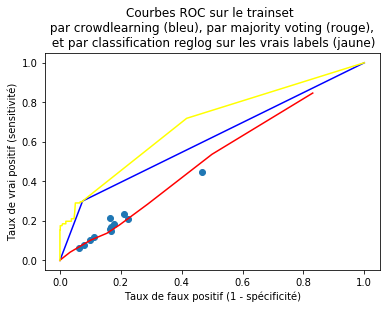
\includegraphics[scale=0.85]{DonneesRellesROC.png}
    \caption{VraisLabels}
    \label{fig:my_label}
\end{figure}

    \end{minipage}

    \begin{minipage}{1.49\textwidth}

\begin{figure}
\vspace{-11cm}
    \centering
    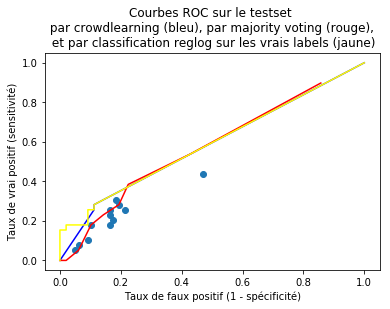
\includegraphics[scale=0.85]{DonneesRellesROCTest.png}
    \caption{VraisLabels}
    \label{fig:my_label}
\end{figure}

    \end{minipage}
\end{block}

%----------------------------------------------------------------------------------------
%	REFERENCES
%----------------------------------------------------------------------------------------
\vspace{-1cm}
\begin{block}{Bibliographie}

  \begin{minipage}{0.8\textwidth}
    \begin{itemize}
      \small
        \item Yan Yan, Gerardo Hermosillo - \textit{Modeling annotator expertise: Learning when everybody know a bit of something}
        \item Vikas C. Raykar, ShipengYu - \textit{Learning from the crowd}
        \item UCI Machine Learning - \textit{"Adult"} datasets

    \end{itemize}
    \end{minipage}

    \begin{minipage}{1.49\textwidth}

  \begin{center}

      \vspace{-4cm}
      \hspace{6cm}
      \includegraphics[scale=0.16]{logos.png}
  \end{center}
    \end{minipage}
\end{block}

%----------------------------------------------------------------------------------------

\end{column} % End of the third column

\end{columns} % End of all the columns in the poster

\end{frame} % End of the enclosing frame

\end{document}
